\documentclass[12pt,a4paper]{report}

% Packages
\usepackage[margin=1in]{geometry}
\usepackage{setspace}
\usepackage{graphicx}
\usepackage{titlesec}
\usepackage{fancyhdr}
\usepackage{tocloft}
\usepackage{rotating}
\usepackage{float}
\usepackage{afterpage}

% Line spacing
\onehalfspacing

% Header & Footer
\pagestyle{fancy}
\fancyhf{}
\rhead{ChatFlow}
\lhead{Software Engineering Project}
\rfoot{\thepage}

% Title formatting
\titleformat{\chapter}[display]
  {\normalfont\huge\bfseries}{\chaptername\ \thechapter}{20pt}{\Huge}

\begin{document}

% ---------------- TITLE PAGE ----------------
\begin{titlepage}
    \centering

    {\Huge \textbf{ChatFlow — Learn, Chat, Flow} \par}
    \vspace{1.5cm}

    {\Large Software Engineering Project Report \par}
    \vspace{1.5cm}

    \textbf{Submitted By:} \\
    Group-7 \\
    202451129 - Shivang Patel \\
    202451130 - Piyush Satiya \\
    202451131 - Piyush Singh \\
    202451146 - Saksham Bansal\\

    \vspace{0.5cm}

    \textbf{Under the Guidance of:} \\
    Dr. Pooja Mishra \\

    \vspace{0.5cm}

    \textbf{Indian Institute of Information Technology, Vadodara} \\
    \begin{figure}[h]
    \centering
    \includegraphics[width=0.5\textwidth]{images.png}
\end{figure}
    \textbf{Department of Computer Science} \\

    \vfill

    \textbf{Date:} \today

\end{titlepage}

% ---------------- ABSTRACT ----------------
\chapter*{Abstract}
\addcontentsline{toc}{chapter}{Abstract}

% Write abstract here

% ---------------- TABLE OF CONTENTS ----------------
\tableofcontents
\newpage

% ---------------- INTRODUCTION ----------------
\chapter{Introduction}

\section{Project Overview}

ChatFlow is a real-time web-based chat application developed as a full-stack Software Engineering project. The system enables users to communicate instantly through text messages and media sharing using a modern and responsive web interface. 

The application is designed using a client-server architecture, where the frontend is built using React and the backend is developed using Node.js and Express. Real-time communication is achieved using WebSocket technology through Socket.io, allowing users to exchange messages without page refresh.

The system also integrates MongoDB as a NoSQL database for persistent data storage and Cloudinary for handling media uploads. ChatFlow provides essential communication features such as user authentication, real-time messaging, online user tracking, and profile management.

\section{Purpose}

The primary purpose of developing ChatFlow is to design and implement a scalable and efficient real-time communication system while applying core concepts of Software Engineering.

This project serves multiple objectives:

\begin{itemize}
    \item To understand and implement full-stack web development using modern technologies.
    \item To explore real-time communication using WebSockets.
    \item To implement secure authentication mechanisms using JSON Web Tokens (JWT).
    \item To design a system with modular architecture and maintainable code structure.
    \item To gain practical experience in integrating third-party services such as Cloudinary.
\end{itemize}

Additionally, this document serves as a reference for understanding system requirements, design decisions, and implementation details for academic evaluation.

\section{Scope}

The scope of ChatFlow is limited to a web-based real-time chat application that supports communication between registered users.

The system provides the following functionalities:

\begin{itemize}
    \item User registration and login with secure authentication.
    \item Real-time one-to-one messaging between users.
    \item Persistent storage of chat messages.
    \item Online and offline user status tracking.
    \item Image and media sharing within chat.
    \item Profile management including profile picture and bio updates.
\end{itemize}

The application is accessible through modern web browsers and is designed to work across different screen sizes with a responsive interface.

However, the current system does not include advanced features such as group chats, voice/video calling, or end-to-end encryption.

\section{Issues}

Despite achieving the core objectives, certain challenges and limitations were encountered during the development of ChatFlow.

\subsection{Technical Challenges}

\begin{itemize}
    \item Ensuring real-time message delivery to the correct user without broadcasting to all connected clients.
    \item Managing synchronization of unseen message counts across different states.
    \item Handling large image uploads efficiently using base64 encoding.
    \item Maintaining socket connections and avoiding memory leaks in event listeners.
\end{itemize}

\subsection{System Limitations}

\begin{itemize}
    \item The system currently supports only one-to-one messaging and does not include group chat functionality.
    \item There is no implementation of end-to-end encryption for messages.
    \item JWT tokens do not have an expiration mechanism in the current version.
    \item The system relies on continuous internet connectivity.
\end{itemize}

\subsection{Future Considerations}

These issues highlight areas for improvement and provide direction for future enhancements such as scalability improvements, enhanced security, and additional communication features.

% ---------------- REQUIREMENT ANALYSIS ----------------
\chapter{Requirement Analysis}

Requirement analysis is a crucial phase in the Software Development Life Cycle (SDLC) where the needs and expectations of the system are identified and documented. For the ChatFlow application, requirements are categorized into functional and non-functional requirements.

\section{Functional Requirements}

Functional requirements define the core functionalities and operations that the system must perform. These requirements describe how the system behaves in response to user actions.

\subsection{User Authentication}

\begin{itemize}
    \item The system shall allow users to register by providing their name, email, password, and bio.
    \item The system shall ensure that each email address is unique.
    \item The system shall securely store user passwords using hashing techniques.
    \item The system shall allow registered users to log in using valid credentials.
    \item The system shall generate and return a JWT token upon successful authentication.
    \item The system shall restrict access to protected routes for unauthenticated users.
    \item The system shall allow users to log out and terminate their session.
\end{itemize}

\subsection{User Profile Management}

\begin{itemize}
    \item The system shall allow users to view and update their profile information.
    \item The system shall allow users to upload and update profile pictures.
    \item The system shall store profile images using cloud-based storage.
    \item The system shall display user details such as name, bio, and profile picture.
\end{itemize}

\subsection{Messaging System}

\begin{itemize}
    \item The system shall support real-time one-to-one messaging between users.
    \item The system shall store all messages persistently in the database.
    \item Each message shall include sender, receiver, timestamp, and content.
    \item The system shall allow users to send text messages and images.
    \item The system shall display messages in chronological order.
\end{itemize}

\subsection{Real-Time Communication}

\begin{itemize}
    \item The system shall establish a real-time connection using WebSockets after login.
    \item The system shall deliver messages instantly to online users.
    \item The system shall update message status dynamically without page refresh.
    \item The system shall notify users about new incoming messages in real time.
\end{itemize}

\subsection{Online Presence Tracking}

\begin{itemize}
    \item The system shall maintain a list of currently online users.
    \item The system shall update user status when they connect or disconnect.
    \item The system shall display online/offline indicators in the user interface.
\end{itemize}

\subsection{Unseen Message Tracking}

\begin{itemize}
    \item The system shall track messages that have not been viewed by the receiver.
    \item The system shall display the count of unseen messages for each user.
    \item The system shall mark messages as seen when the conversation is opened.
\end{itemize}

\subsection{Media Sharing}

\begin{itemize}
    \item The system shall allow users to upload and send image files in chats.
    \item The system shall validate file types before uploading.
    \item The system shall store media files externally and maintain their URLs in the database.
\end{itemize}

\section{Non-Functional Requirements}

Non-functional requirements define the quality attributes of the system such as performance, security, scalability, and usability.

\subsection{Performance}

The system must ensure efficient and fast message delivery with minimal latency. Real-time communication should be smooth and responsive. The system should handle multiple users simultaneously without degradation in performance.

\subsection{Security}

The system must ensure data security and user privacy. Passwords must be encrypted using secure hashing algorithms. Authentication must be handled using JWT tokens. Unauthorized access to protected resources must be prevented. Sensitive information such as API keys and database credentials must be stored securely.

\subsection{Scalability}

The system should be designed to handle increasing numbers of users and messages. The use of stateless authentication and cloud-based services allows the system to scale horizontally when needed.

\subsection{Usability}

The application must provide an intuitive and user-friendly interface. Navigation should be simple and responsive across different devices. The system should provide feedback to user actions through notifications and visual indicators.

\subsection{Reliability}

The system must ensure that messages are not lost during transmission. Data consistency must be maintained in the database. The system should handle unexpected errors gracefully.

\subsection{Maintainability}

The application should follow a modular design approach, making it easier to update and maintain. Code should be well-structured and follow best practices to allow future enhancements.

\subsection{Availability}

The system should be accessible at all times with minimal downtime. It should depend on stable backend services and database connectivity.

% ---------------- DESIGN AND ARCHITECTURE ----------------
\chapter{Design and Architecture}

This chapter describes the design aspects of the ChatFlow system, including its architecture, data flow, module structure, and database design. The system is designed using a modular approach to ensure scalability, maintainability, and efficient performance.

\section{System Architecture}

ChatFlow follows a client-server architecture where the frontend and backend communicate through REST APIs and WebSocket connections.

\begin{itemize}
    \item \textbf{Frontend:} Built using React, responsible for handling user interactions and rendering UI components.
    \item \textbf{Backend:} Developed using Node.js and Express, which processes requests and handles business logic.
    \item \textbf{Database:} MongoDB is used to store user data and messages.
    \item \textbf{Media Storage:} Cloudinary is used for storing and serving images.
\end{itemize}

The system uses HTTP for API communication and WebSocket (Socket.io) for real-time messaging.

\section{Data Flow Diagram (Level 2)}

The Data Flow Diagram (DFD Level 2) provides a detailed representation of how data flows through different processes within the system.

% \begin{figure}[h]
%     \centering
%     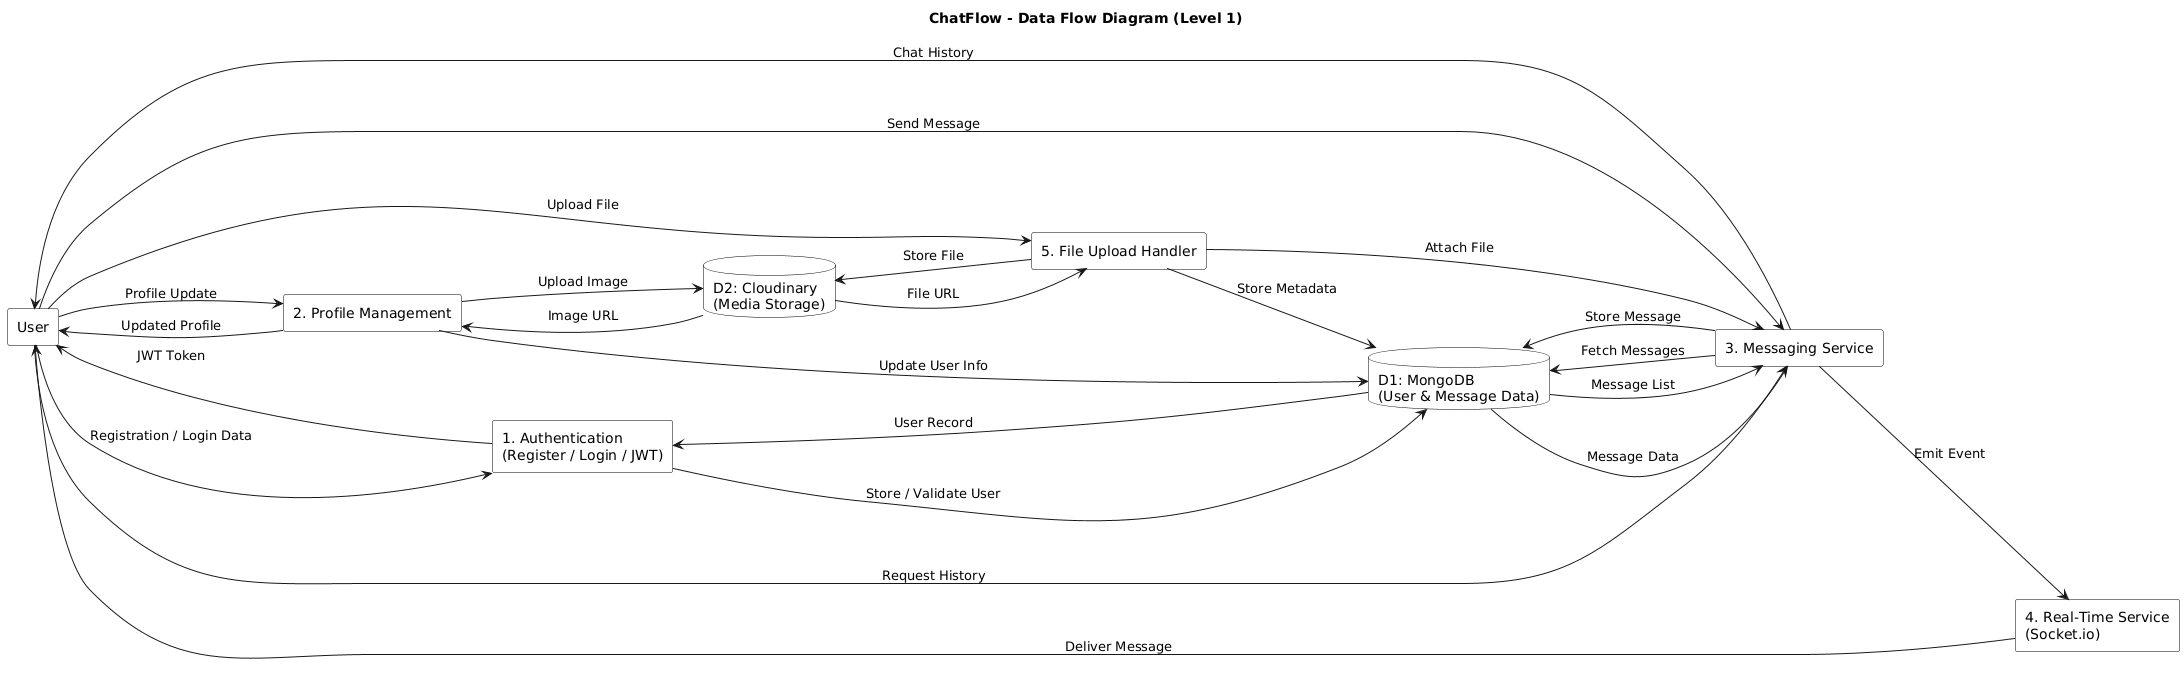
\includegraphics[width=0.85\textwidth]{dataflowDiagram.png}
%     \caption{Data Flow Diagram (Level 2) of ChatFlow}
% \end{figure}
% \begin{sidewaysfigure}
%     \centering
%     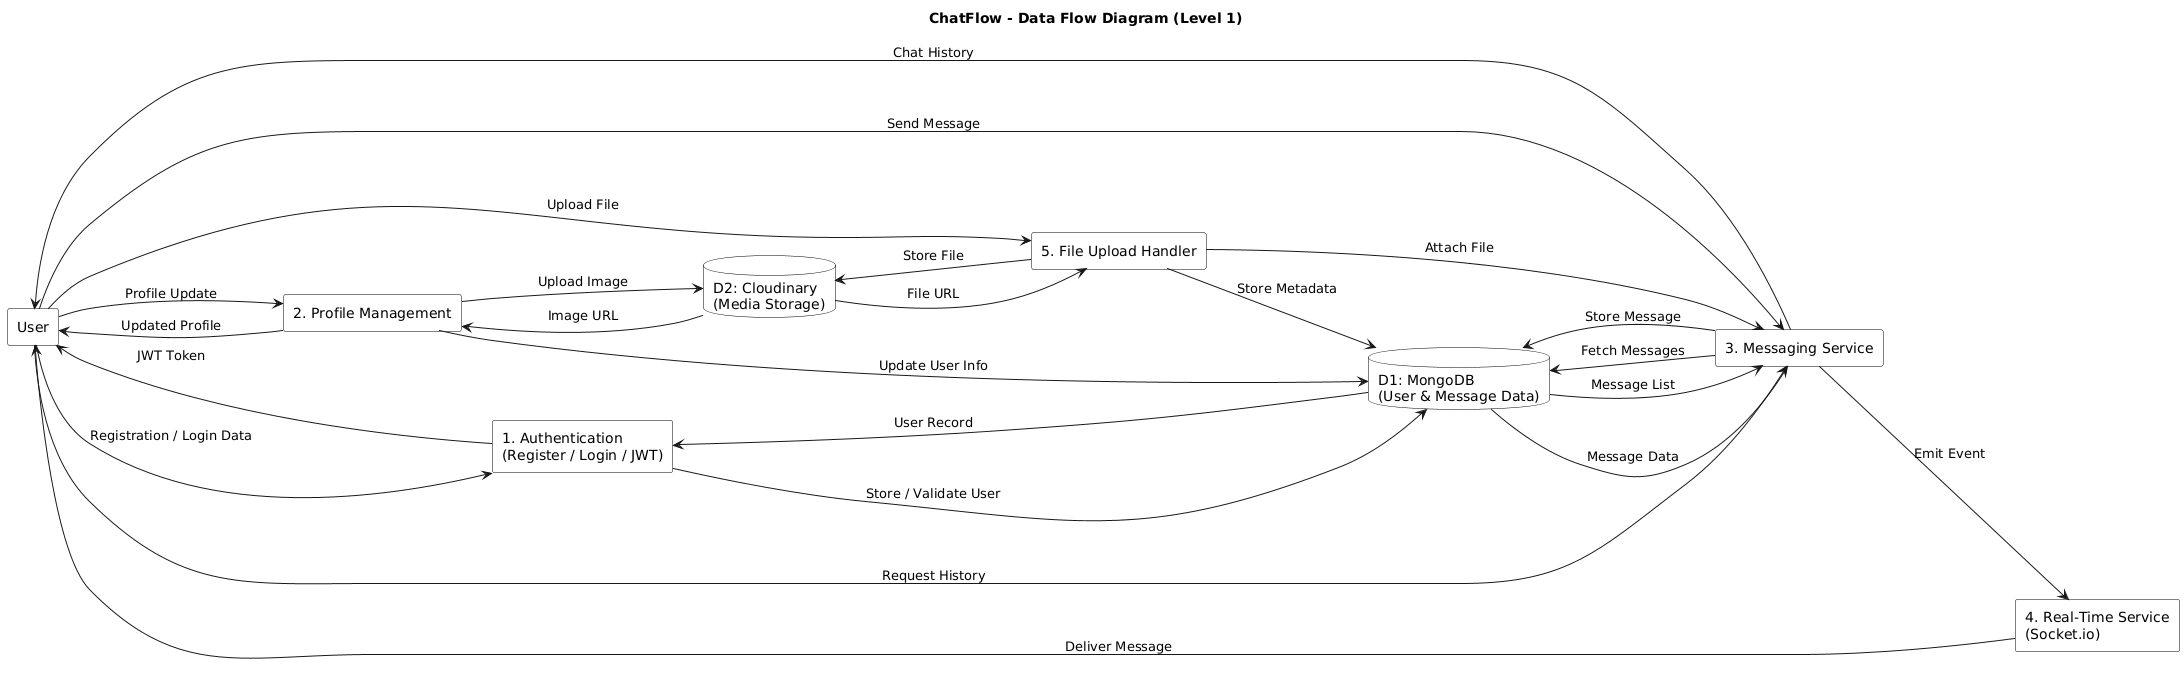
\includegraphics[width=\textheight]{dataflowDiagram.png}
%     \caption{Data Flow Diagram (Level 2) of ChatFlow}
% \end{sidewaysfigure}
\begin{figure}[p]
    \centering
    \rotatebox{90}{
        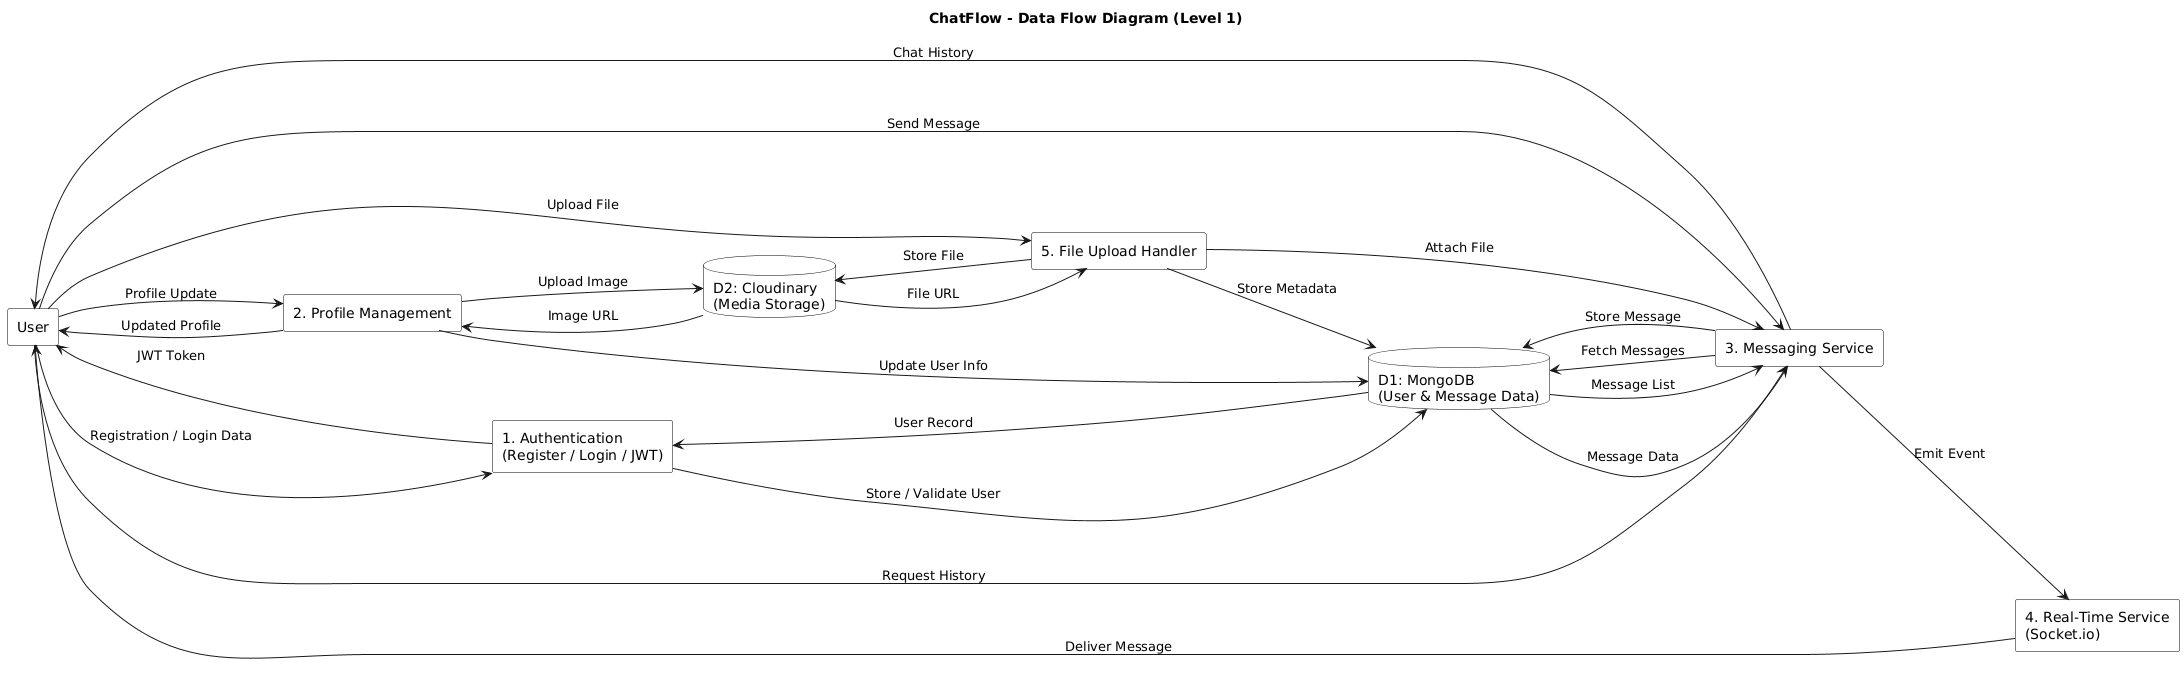
\includegraphics[width=0.9\textheight]{dataflowDiagram.png}
    }
    \caption{Data Flow Diagram (Level 2) of ChatFlow}
\end{figure}

The diagram illustrates internal processes such as authentication, message handling, media upload, and database interactions.

\section{Use Case Diagram}

The Use Case Diagram represents the interaction between the user and the system functionalities.

% \begin{figure}[h]
%     \centering
%     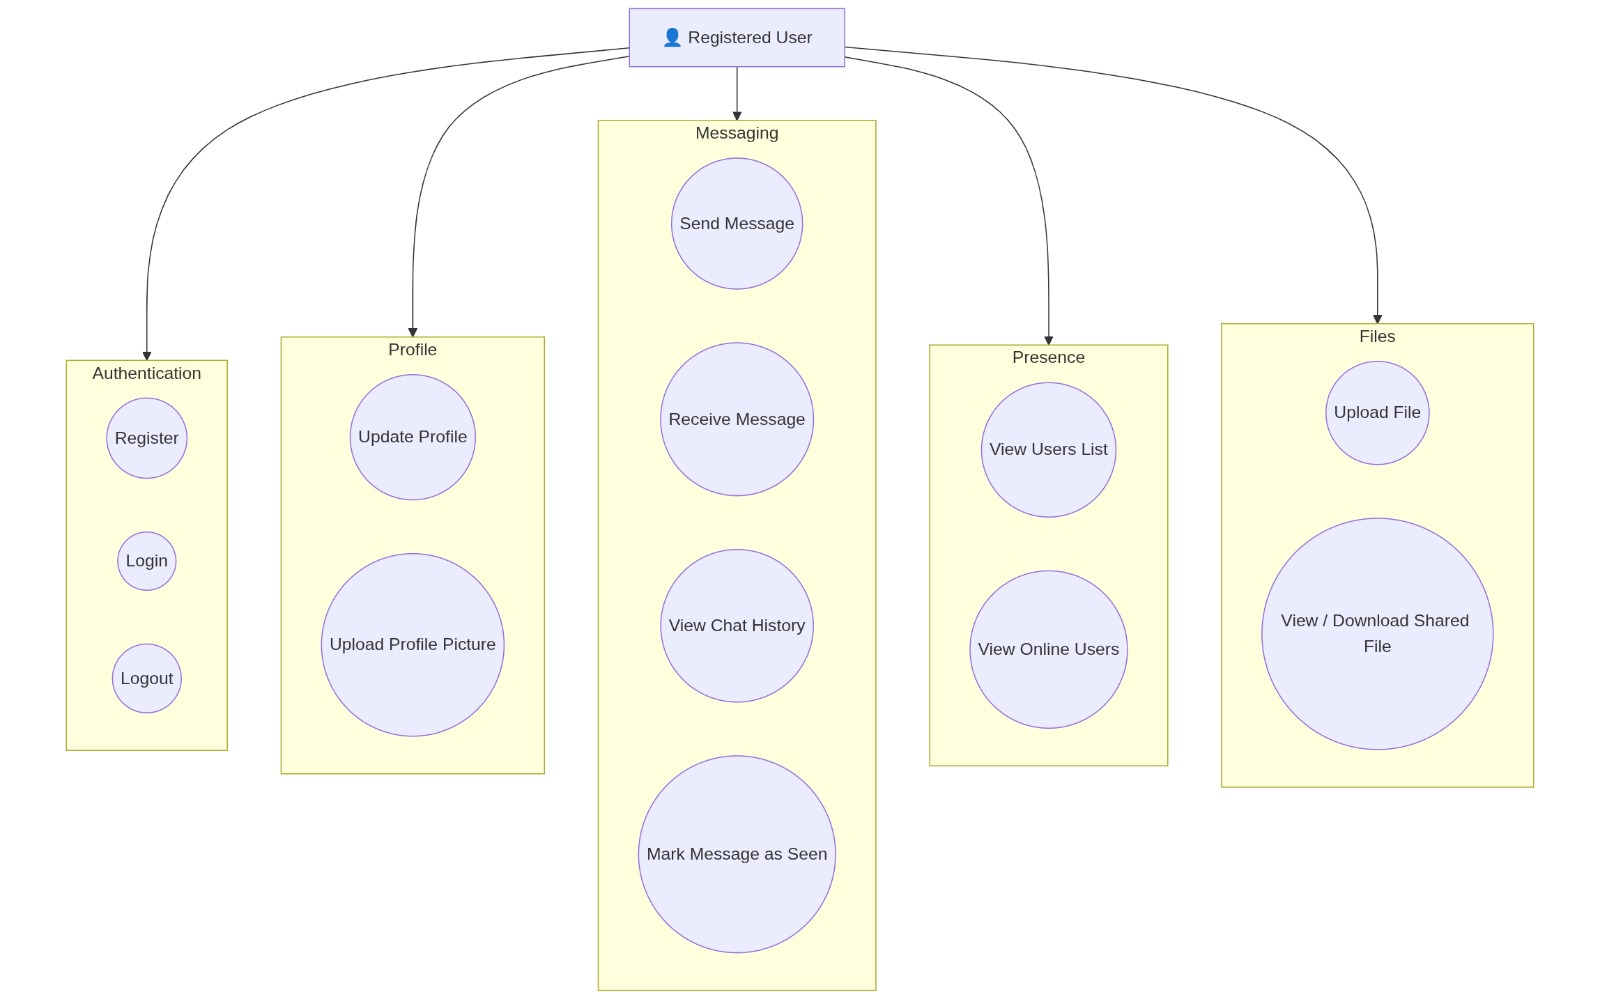
\includegraphics[width=0.75\textwidth]{useCase.jpeg}
%     \caption{Use Case Diagram of ChatFlow}
% \end{figure}
% \begin{sidewaysfigure}
%     \centering
%     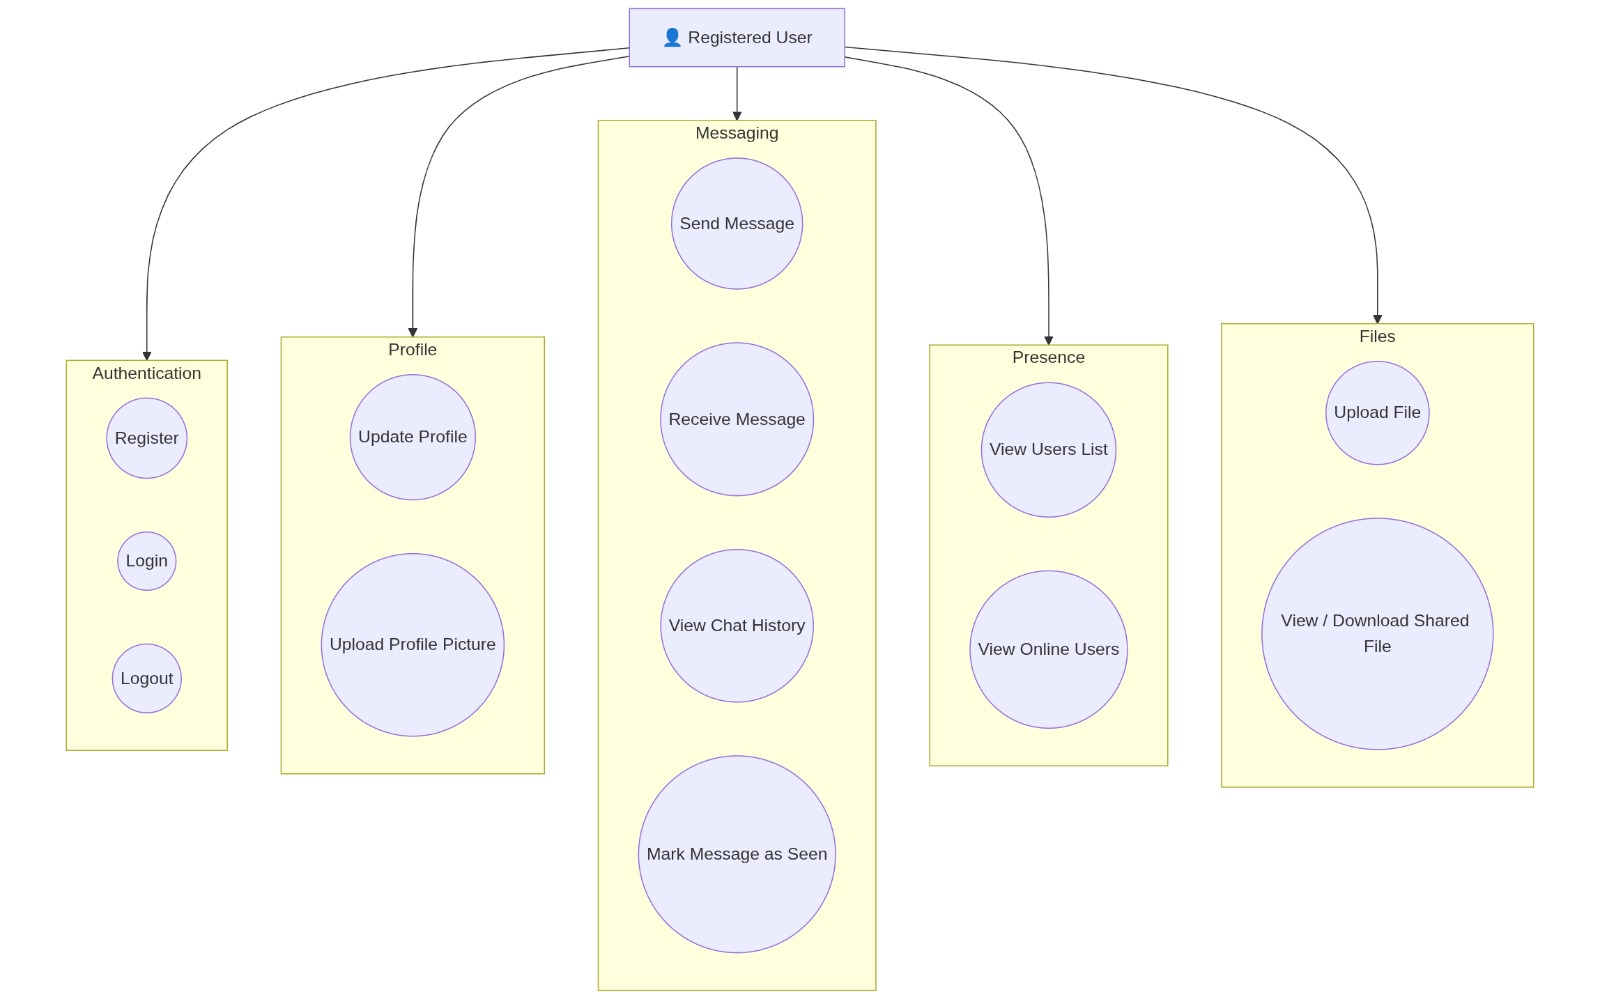
\includegraphics[width=\textheight]{useCase.jpeg}
%     \caption{Data Flow Diagram (Level 2) of ChatFlow}
% \end{sidewaysfigure}

The primary actor in the system is the registered user. The user can perform actions such as registering, logging in, sending messages, receiving messages, updating profile, and viewing chat history.

\clearpage
\begin{figure}[p]
    \centering
    \rotatebox{90}{
        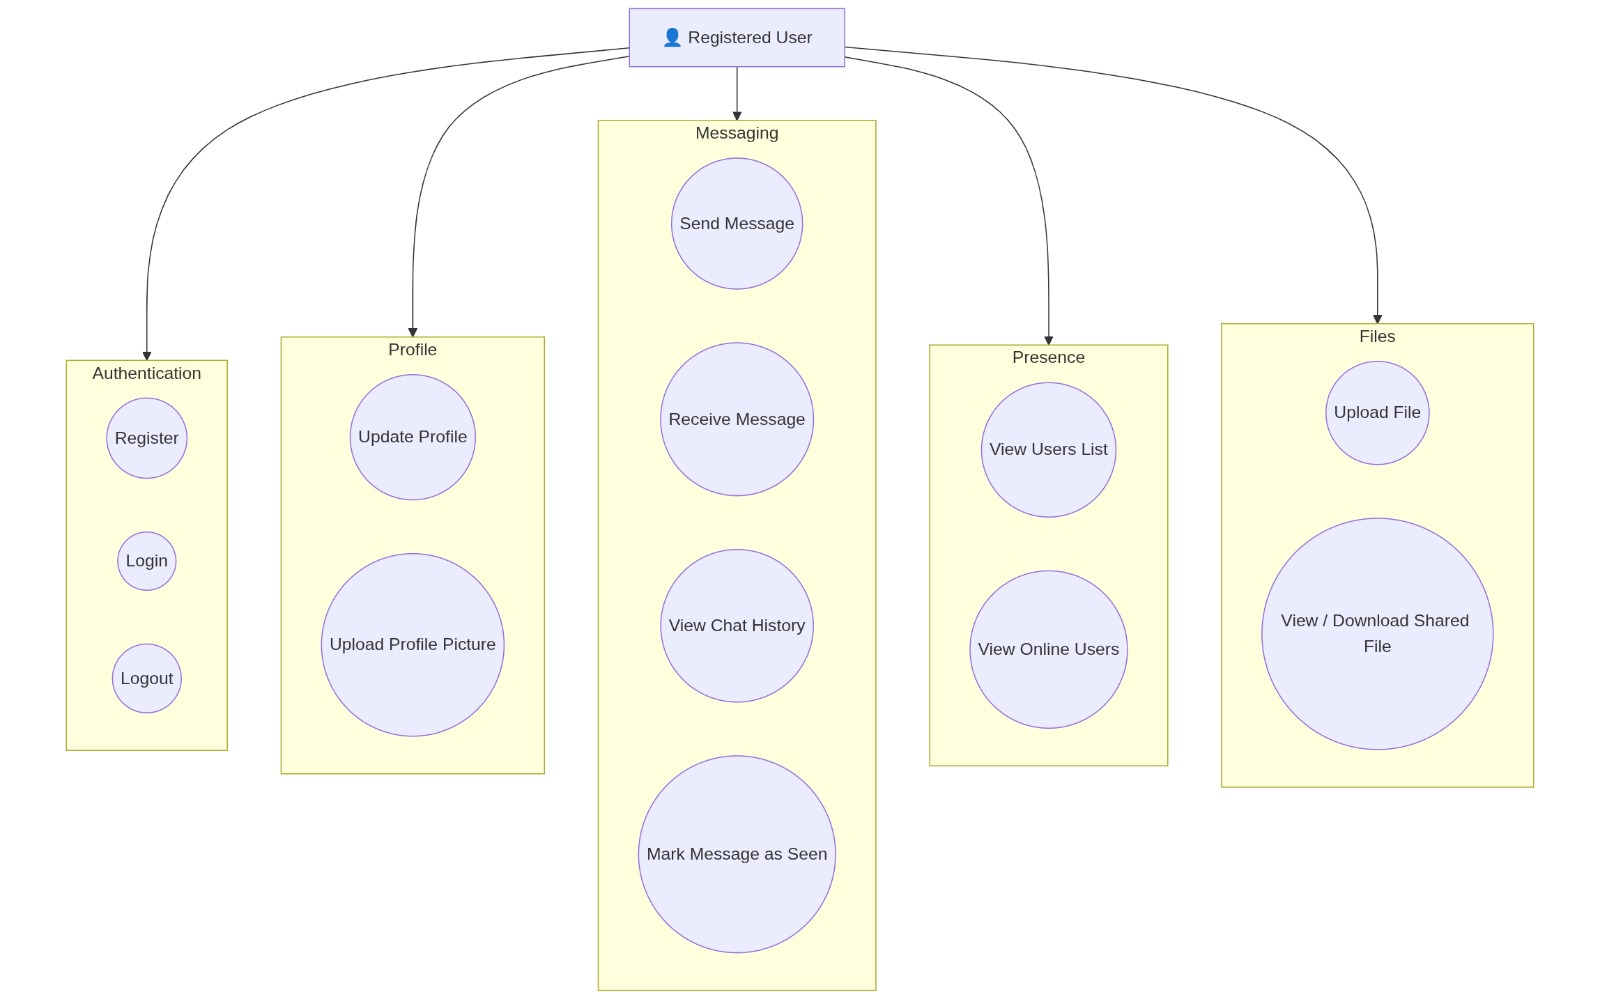
\includegraphics[width=0.9\textheight]{useCase.jpeg}
    }
    \caption{Use Case Diagram of ChatFlow}
\end{figure}
\clearpage

\section{Class Diagram}

The Class Diagram represents the static structure of the system, including classes, attributes, and relationships.

% \begin{figure}[h]
%     \centering
%     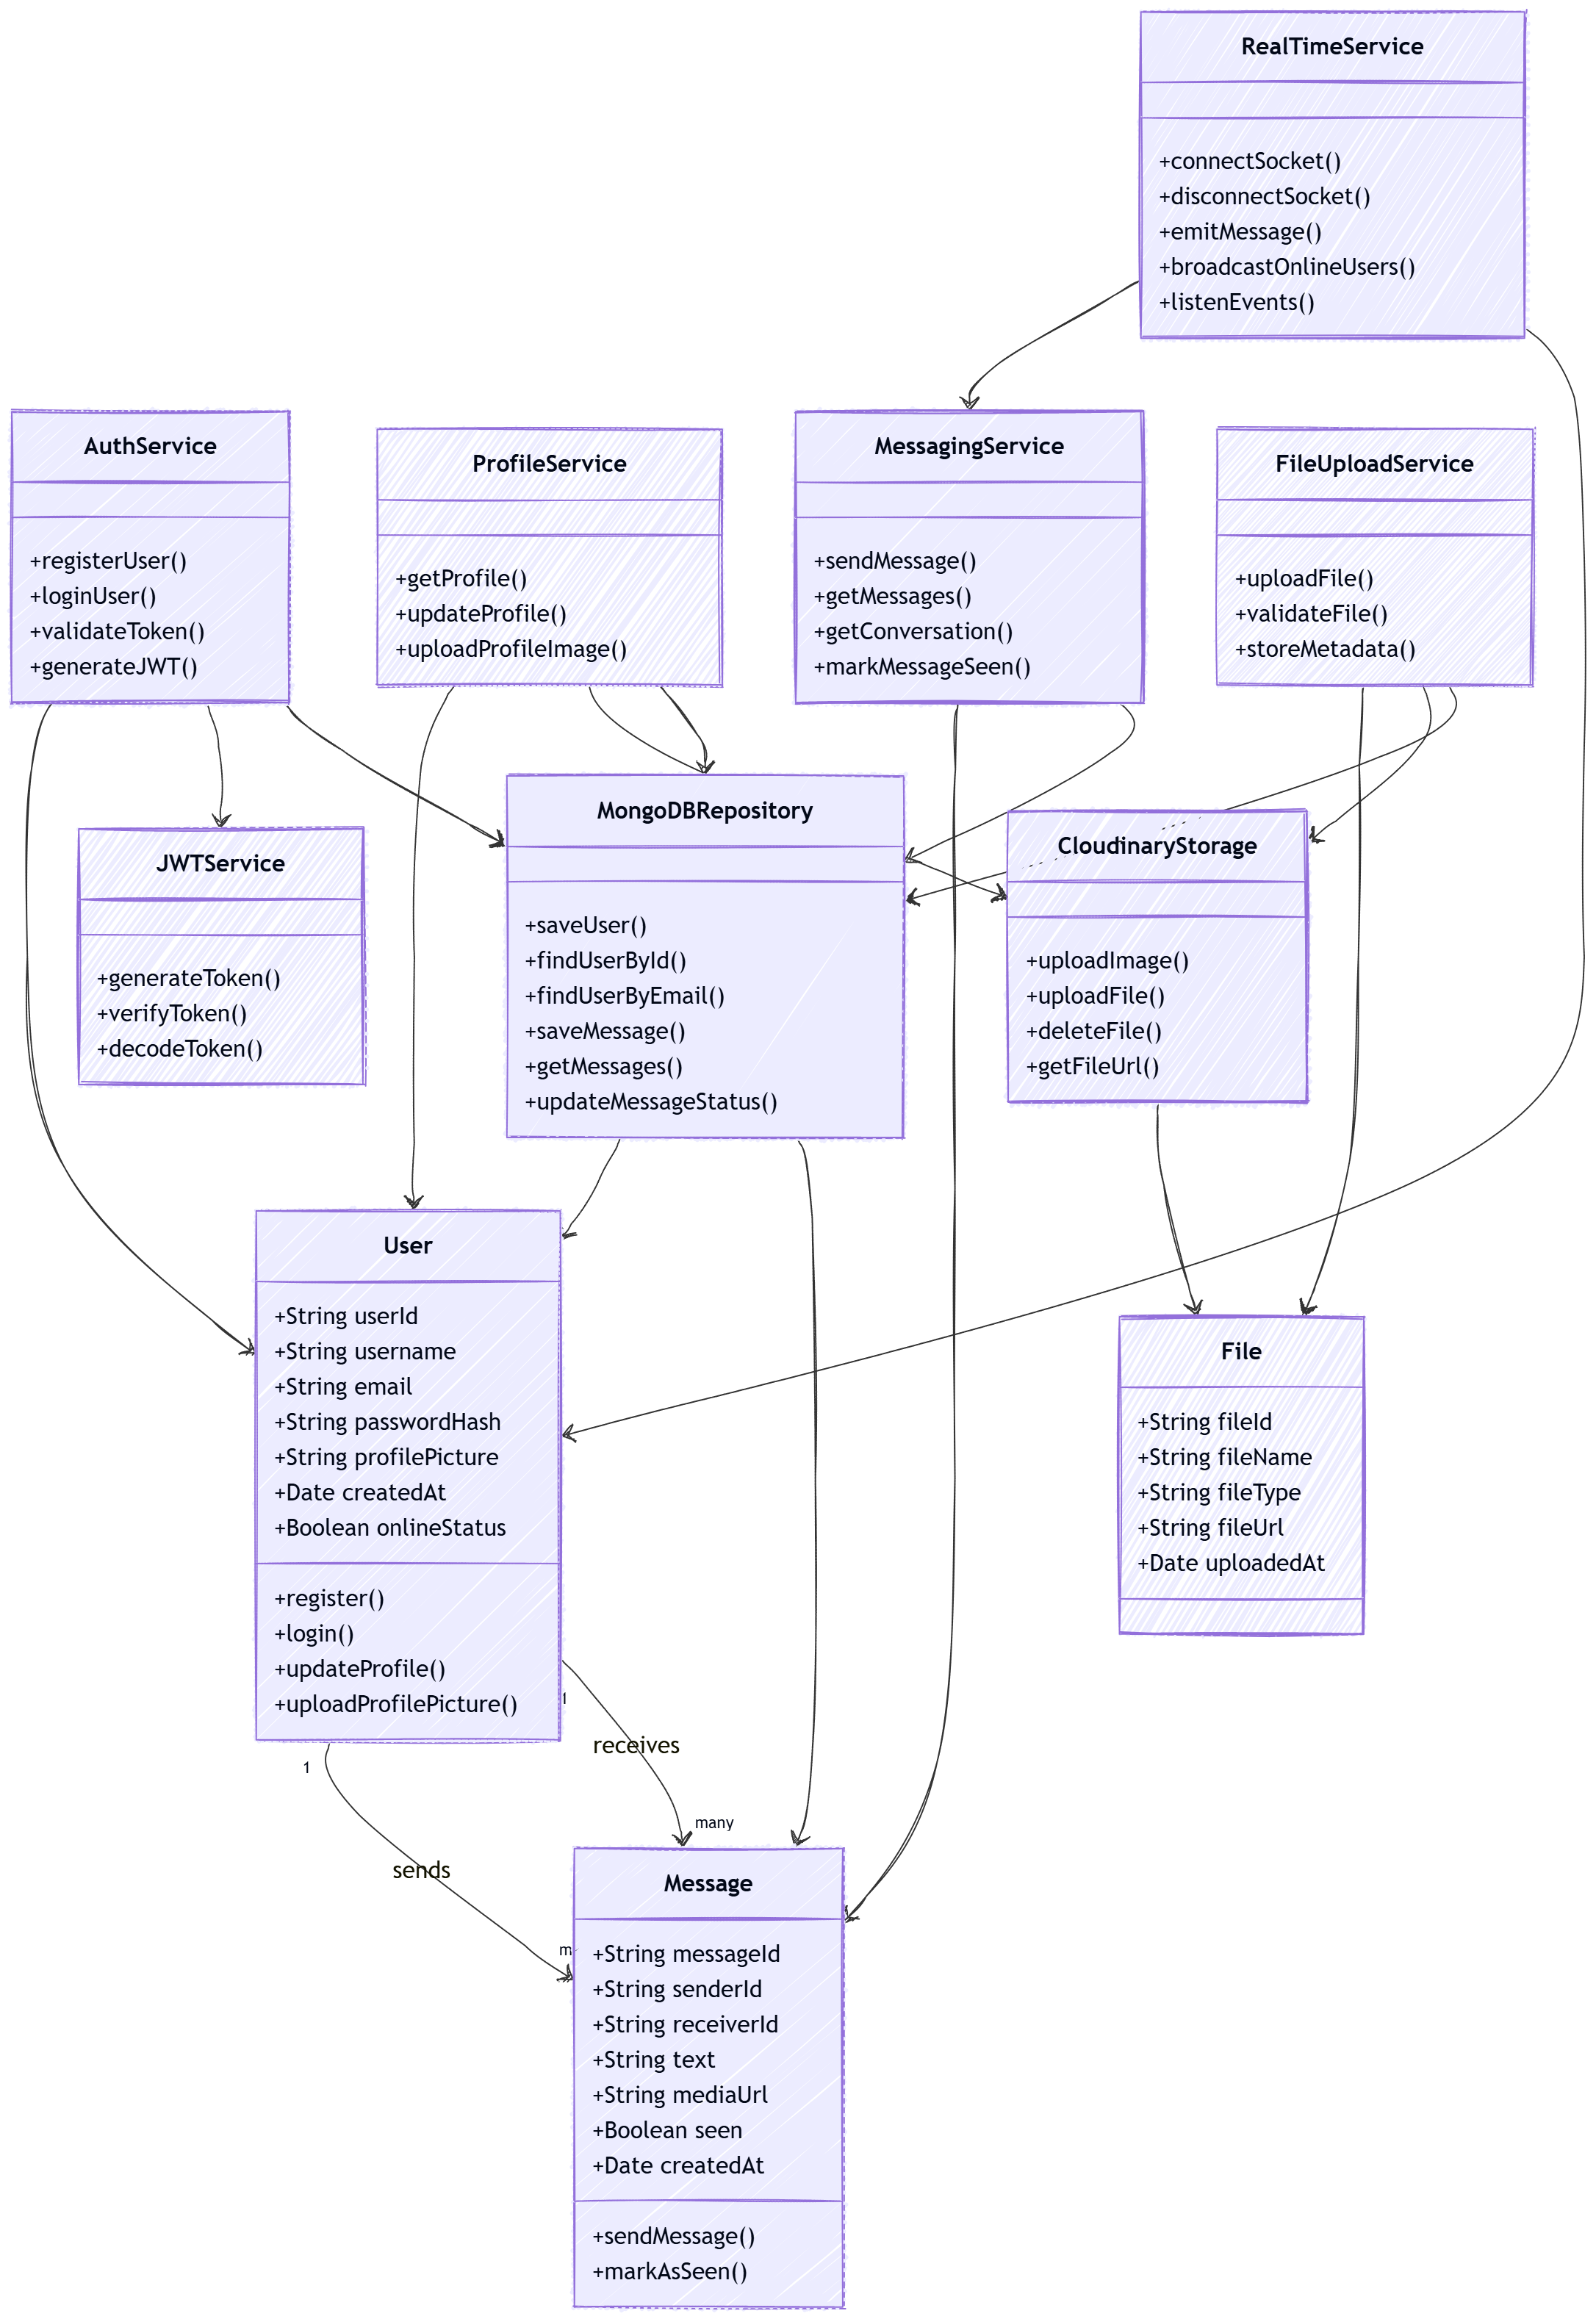
\includegraphics[width=1\textwidth]{classDiagram.png}
%     \caption{Class Diagram of ChatFlow}
% \end{figure}
% \begin{figure}[H]
%     \centering
%     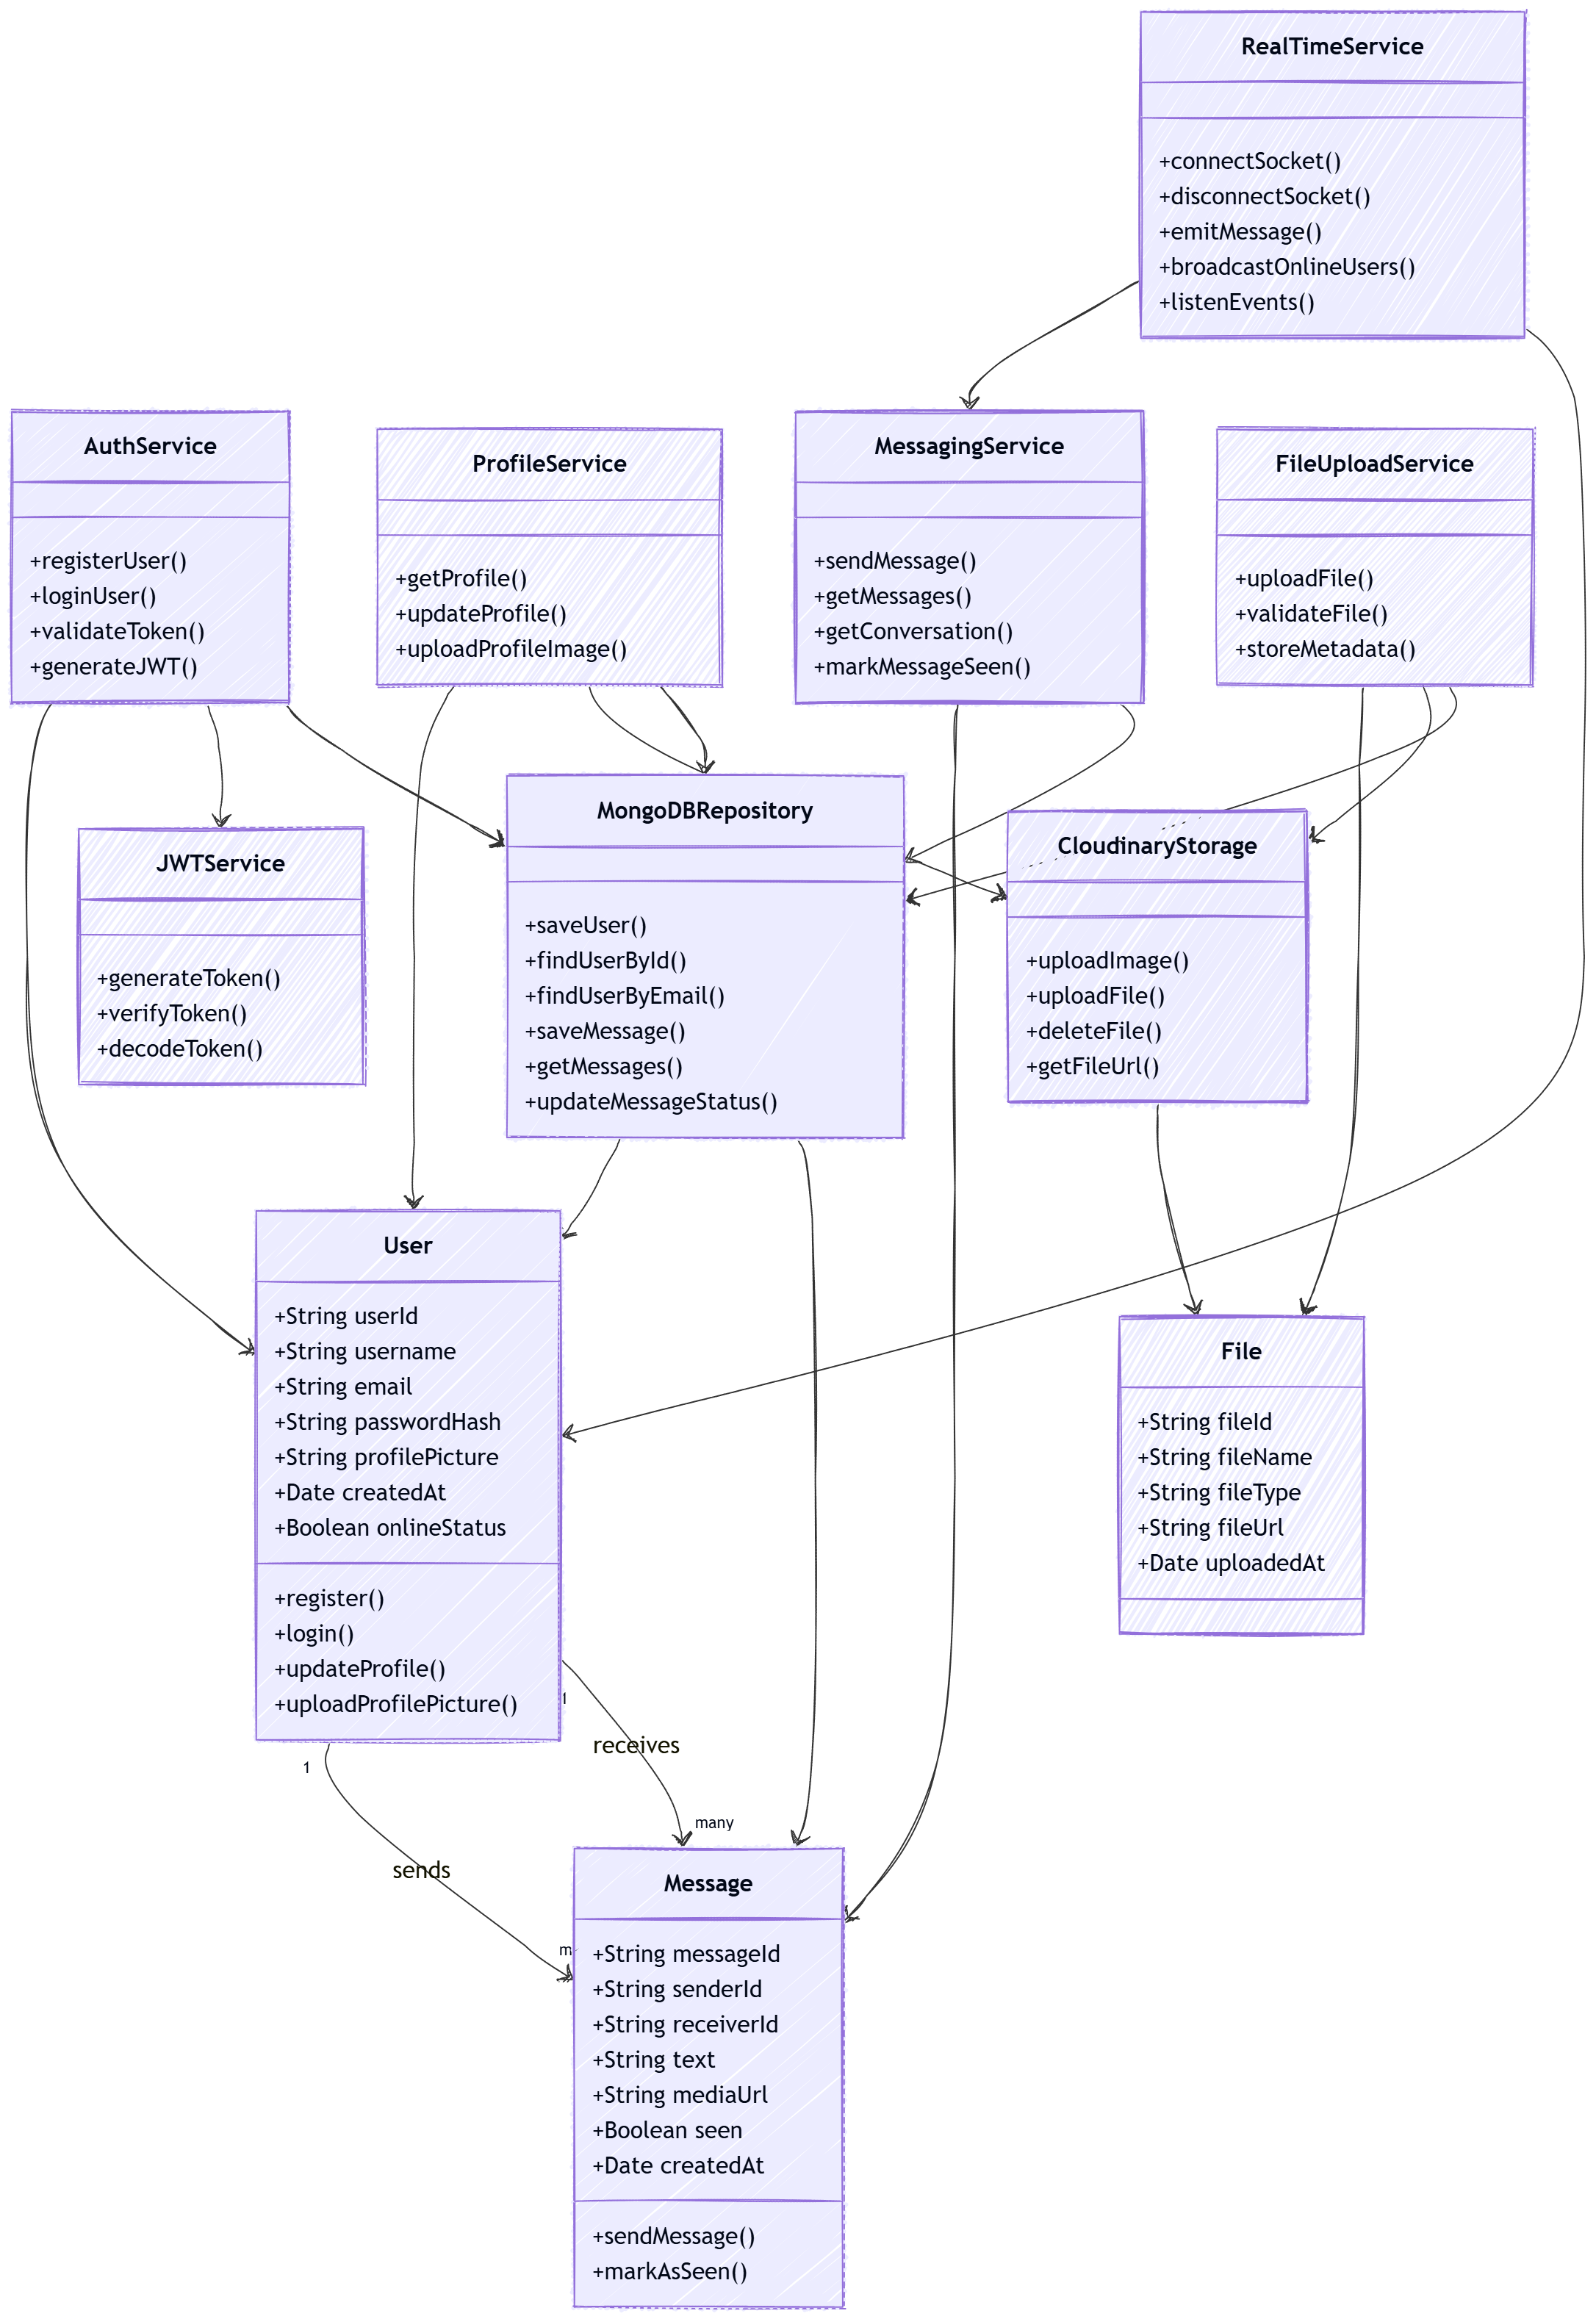
\includegraphics[width=\textwidth,height=0.9\textheight,keepaspectratio]{classDiagram.png}
%     \caption{Class Diagram of ChatFlow}
% \end{figure}

The main classes in the system include:

\begin{itemize}
    \item \textbf{User Class:} Contains attributes such as userId, name, email, password, profile picture, and bio.
    \item \textbf{Message Class:} Contains attributes such as messageId, senderId, receiverId, content, media URL, timestamp, and seen status.
\end{itemize}

The relationship between these classes defines how users interact through messages in the system.

\clearpage
\begin{figure}[p]
    \centering
    % \rotatebox{90}{
        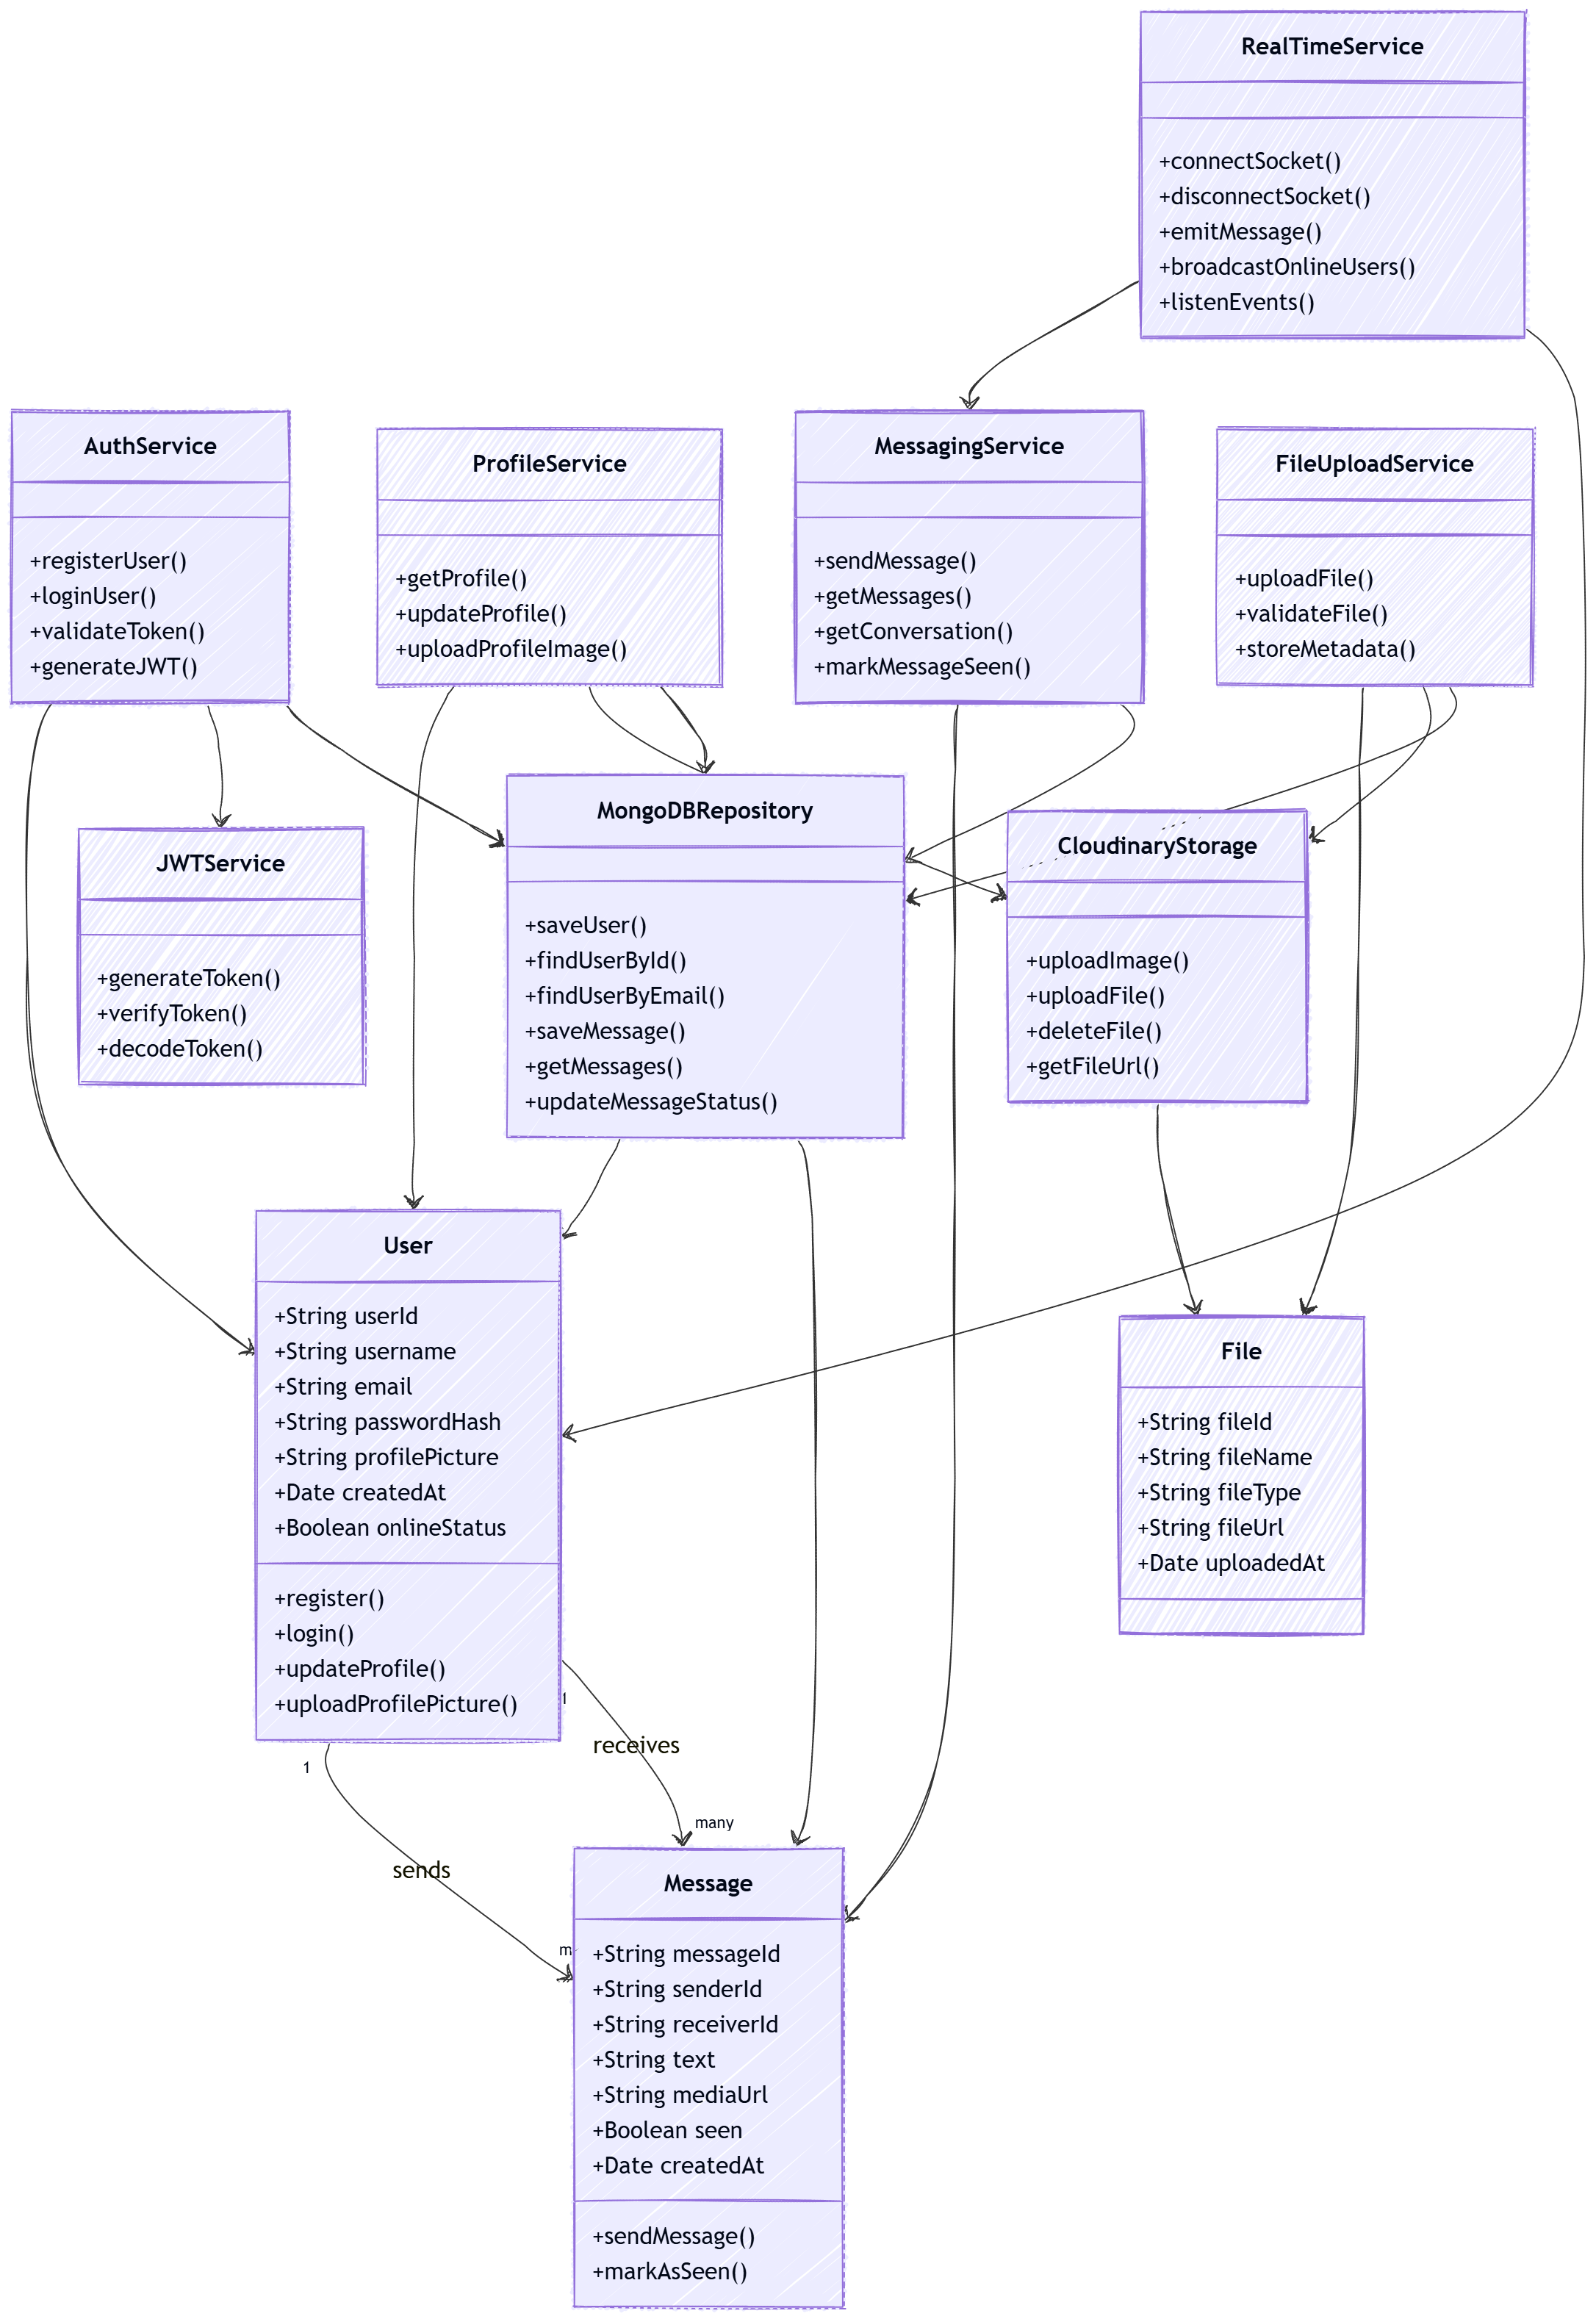
\includegraphics[width=\textwidth]{classDiagram.png}
    % }
    \caption{Use Case Diagram of ChatFlow}
\end{figure}
\clearpage

\section{Module Design}

The system is divided into different modules to ensure separation of concerns.

\subsection{Authentication Module}
Handles user registration, login, logout, and authentication using JWT tokens.

\subsection{Messaging Module}
Manages sending, receiving, and storing messages, including real-time delivery.

\subsection{Real-Time Communication Module}
Uses Socket.io to enable instant communication and track online users.

\subsection{Profile Management Module}
Allows users to update personal details such as name, bio, and profile picture.

\subsection{Media Handling Module}
Handles image uploads and integrates with Cloudinary for storage and retrieval.

\section{Database Design}

The system uses MongoDB to manage data in a flexible and scalable way.

\subsection{Entity Relationship Diagram}
\clearpage
\begin{figure}[p]
    \centering
    % \rotatebox{90}{
        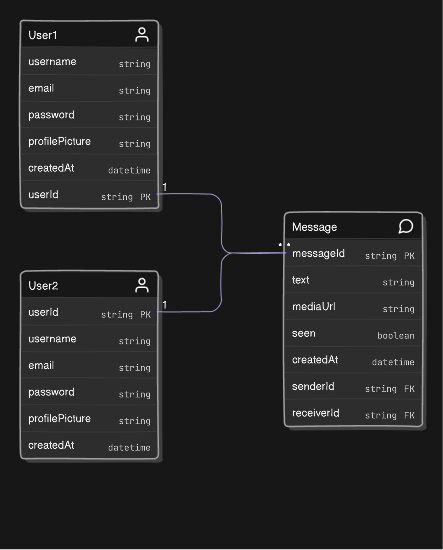
\includegraphics[width=\textwidth]{er_diagram.jpeg}
    % }
    \caption{Use Case Diagram of ChatFlow}
\end{figure}
\clearpage

% \begin{figure}
%     \centering
%     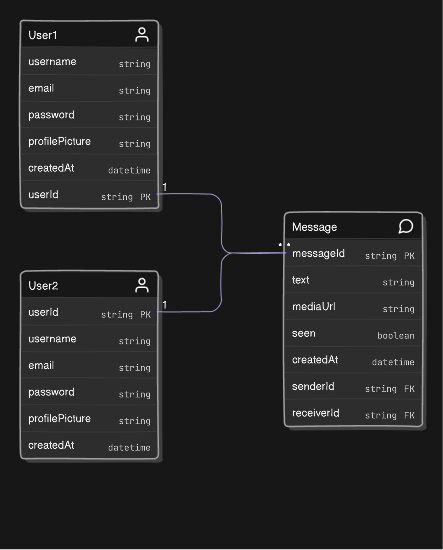
\includegraphics[width=\textheight]{er_diagram.jpeg}
%     \caption{Data Flow Diagram (Level 2) of ChatFlow}
% \end{figure}


% \begin{figure}[h]
%     \centering
%     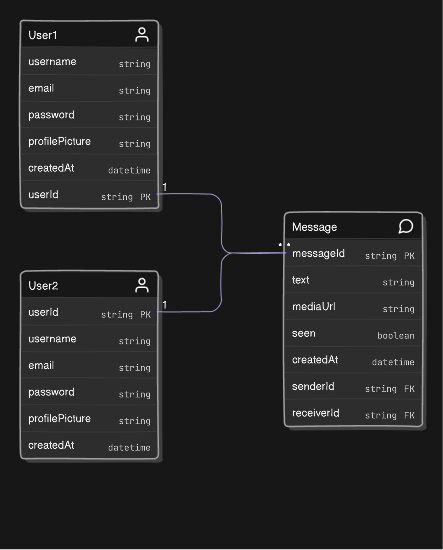
\includegraphics[width=0.8\textwidth]{er_diagram.jpeg}
%     \caption{Entity Relationship Diagram of ChatFlow}
% \end{figure}

\subsection{Entities Description}

\textbf{User Entity:}
Stores user information such as name, email, password, profile picture, and bio.

\textbf{Message Entity:}
Stores messages exchanged between users, including sender, receiver, content, media URL, and seen status.

\subsection{Relationships}

\begin{itemize}
    \item One user can send multiple messages.
    \item One user can receive multiple messages.
    \item Each message is associated with one sender and one receiver.
\end{itemize}


% ---------------- IMPLEMENTATION DETAILS ----------------
\chapter{Implementation Details}

\section{Technologies Used}
The ChatFlow application is implemented as a full-stack JavaScript system with clearly separated frontend and backend layers.

\subsection{Frontend Technologies}
\begin{itemize}
    \item \textbf{React (v19):} used for component-based UI development and client-side rendering.
    \item \textbf{React Router:} used for route-level access control between login, home, and profile pages.
    \item \textbf{Axios:} used for HTTP communication with backend APIs.
    \item \textbf{Socket.io Client:} used to subscribe to real-time events such as new messages and online users.
    \item \textbf{Tailwind CSS:} used for responsive styling and modern UI layouts.
\end{itemize}

\subsection{Backend Technologies}
\begin{itemize}
    \item \textbf{Node.js and Express:} used to implement REST APIs and server-side business logic.
    \item \textbf{Socket.io:} used for bidirectional real-time communication.
    \item \textbf{JWT (jsonwebtoken):} used for stateless authentication.
    \item \textbf{bcryptjs:} used to hash and verify user passwords.
\end{itemize}

\subsection{Database and External Services}
\begin{itemize}
    \item \textbf{MongoDB with Mongoose:} used for persisting users and messages.
    \item \textbf{Cloudinary:} used to store profile and chat images and return hosted URLs.
\end{itemize}

\section{Feature Implementation}
This section explains how the main modules were implemented, with direct code references from the ChatFlow repository.

\subsection{Backend Startup, API Binding, and Socket Layer}
The backend initializes Express, creates an HTTP server, mounts API routes, and starts Socket.io for event-driven communication.

\begin{verbatim}
// server/server.js
const app = express();
const server = http.createServer(app);

export const io = new Server(server, {
    cors: { origin: "*" },
});

app.use("/api/status", (req, res) => res.send("server is live"));
app.use("/api/auth", userRouter);
app.use("/api/messages", messageRouter);
\end{verbatim}

The socket layer tracks active users and broadcasts updated presence lists.

\begin{verbatim}
// server/server.js
export const userSocketMap = {}; // {userId: socketId}

io.on("connection", (socket) => {
    const userId = socket.handshake.query.userId;
    if (userId) userSocketMap[userId] = socket.id;

    io.emit("getOnlineUsers", Object.keys(userSocketMap));

    socket.on("disconnect", () => {
        delete userSocketMap[userId];
        io.emit("getOnlineUsers", Object.keys(userSocketMap));
    });
});
\end{verbatim}

\subsection{Database Connection and Schema Design}
MongoDB connection is handled through a dedicated utility module. The service is initialized before server listen flow.

\begin{verbatim}
// server/lib/db.js
const connectDB = async () => {
    try {
        const connectionInstance = await mongoose.connect(
            `${process.env.MONGODB_URI}`
        );

        console.log(
            `DB connected | DB host: ${connectionInstance.connection.host}`
        );
    } catch (error) {
        console.log("Error connecting to DB: ", error.message);
        process.exit(1);
    }
};
\end{verbatim}

The \texttt{User} model defines identity, profile and credential fields:

\begin{verbatim}
// server/models/User.model.js
const userSchema = new mongoose.Schema(
    {
        email: { type: String, required: true, unique: true, lowercase: true, trim: true },
        fullName: { type: String, required: true, trim: true },
        password: { type: String, required: true, trim: true, minlength: 6 },
        profilePic: { type: String, default: "" },
        bio: { type: String, trim: true },
    },
    { timestamps: true }
);
\end{verbatim}

The \texttt{Message} model stores sender-receiver mapping, optional image payload, and seen flag:

\begin{verbatim}
// server/models/message.model.js
const messageSchema = new mongoose.Schema(
    {
        senderId: { type: mongoose.Schema.Types.ObjectId, ref: "User", required: true },
        receiverId: { type: mongoose.Schema.Types.ObjectId, ref: "User", required: true },
        text: { type: String },
        image: { type: String },
        seen: { type: Boolean, default: false },
    },
    { timestamps: true }
);
\end{verbatim}

\subsection{Authentication Flow and Protected Middleware}
Account creation hashes passwords with bcrypt and issues a signed JWT token for stateless sessions.

\begin{verbatim}
// server/controllers/user.controller.js (signup)
const salt = await bcrypt.genSalt(10);
const hashedPassword = await bcrypt.hash(password, salt);

const newUser = await User.create({
    fullName,
    email,
    password: hashedPassword,
    bio,
});

const token = generateToken(newUser._id);
\end{verbatim}

Login verifies credentials by comparing incoming password with the hashed value in database:

\begin{verbatim}
// server/controllers/user.controller.js (login)
const { email, password } = req.body;
const userData = await User.findOne({ email });

const isPasswordCorrect = await bcrypt.compare(
    password,
    userData.password
);

const token = generateToken(userData._id);
\end{verbatim}

Route protection is implemented through JWT verification middleware:

\begin{verbatim}
// server/middlewares/auth.js
const token = req.headers.token;
const decoded = jwt.verify(token, process.env.JWT_SECRET);
const user = await User.findById(decoded.userId).select("-password");

req.user = user;
next();
\end{verbatim}

\subsection{Cloudinary Media Integration}
Cloudinary is configured once at startup and reused in user/message controllers for image uploads.

\begin{verbatim}
// server/lib/cloudinary.js
cloudinary.config({
    cloud_name: process.env.CLOUDINARY_CLOUD_NAME,
    api_key: process.env.CLOUDINARY_API_KEY,
    api_secret: process.env.CLOUDINARY_API_SECRET,
});
\end{verbatim}

Profile image upload flow in controller:

\begin{verbatim}
// server/controllers/user.controller.js (updateProfile)
const upload = await cloudinary.uploader.upload(profilePic);
updateUser = await User.findByIdAndUpdate(
    userId,
    { profilePic: upload.secure_url, bio, fullName },
    { new: true }
);
\end{verbatim}

Chat image upload flow in message controller:

\begin{verbatim}
// server/controllers/message.controller.js (sendMessage)
let imageUrl;
if (image) {
    const uploadResponse = await cloudinary.uploader.upload(image);
    imageUrl = uploadResponse.secure_url;
}
\end{verbatim}

\subsection{Messaging Controller Logic}
The sidebar API computes unseen message counts user-wise using asynchronous queries:

\begin{verbatim}
// server/controllers/message.controller.js (getUserForSidebar)
const filteredUser = await User.find({ _id: { $ne: userId } }).select("-password");
const unseenMessages = {};

await Promise.all(
    filteredUser.map(async (user) => {
        const messages = await Message.find({
            senderId: user._id,
            receiverId: userId,
            seen: false,
        });

        if (messages.length > 0) {
            unseenMessages[user._id] = messages.length;
        }
    })
);
\end{verbatim}

Conversation fetch API returns both directions of messages and marks incoming messages as seen:

\begin{verbatim}
// server/controllers/message.controller.js (getMessages)
const messages = await Message.find({
    $or: [
        { senderId: myId, receiverId: selectedUserId },
        { senderId: selectedUserId, receiverId: myId },
    ],
});

await Message.updateMany(
    { senderId: selectedUserId, receiverId: myId },
    { seen: true }
);
\end{verbatim}

Message sending persists payload and emits only to the target receiver socket:

\begin{verbatim}
// server/controllers/message.controller.js (sendMessage)
const newMessage = await Message.create({
    senderId,
    receiverId,
    text,
    image: imageUrl,
});

const recieversSocketId = userSocketMap[receiverId];
if (recieversSocketId) {
    io.to(recieversSocketId).emit("newMessage", newMessage);
}
\end{verbatim}

\subsection{Routing and Frontend Context Integration}
Backend routes are modular and protected where required:

\begin{verbatim}
// server/routes/userRoutes.js
userRouter.post("/signup", signup);
userRouter.post("/login", login);
userRouter.put("/update-profile", protectedRoute, updateProfile);
userRouter.get("/check", protectedRoute, checkAuth);
\end{verbatim}

\begin{verbatim}
// server/routes/messageRoutes.js
messageRouter.get("/users", protectedRoute, getUserForSidebar);
messageRouter.get("/:id", protectedRoute, getMessages);
messageRouter.put("/mark/:id", protectedRoute, markMessageAsSeen);
messageRouter.post("/send/:id", protectedRoute, sendMessage);
\end{verbatim}

On the frontend, contexts consume these APIs and socket events to keep UI state synchronized in real time.

\begin{verbatim}
// client/context/ChatContext.jsx
const { data } = await axios.get(`/api/messages/${userId}`);
if (data.success) {
    setMessages(data.messages);
}

socket.on("newMessage", (newMessage) => {
    if (selectedUser && newMessage.senderId === selectedUser._id) {
        newMessage.seen = true;
        setMessages((prevMessage) => [...prevMessage, newMessage]);
        axios.put(`/api/messages/mark/${newMessage._id}`);
    }
});
\end{verbatim}

% ---------------- TESTING AND DEPLOYMENT ----------------
\chapter{Testing and Deployment}

\section{Testing}
Testing was performed using \texttt{Vitest} for both backend and frontend modules. The strategy includes unit testing of controllers/models and integration testing for route plus middleware behavior.

\subsection{Backend Testing}
Backend tests validate:
\begin{itemize}
    \item user model and message model constraints,
    \item authentication middleware behavior for valid/invalid JWT,
    \item controller functions for signup/login/profile update,
    \item message operations (send, fetch, mark seen),
    \item route integration using Supertest.
\end{itemize}

Example integration test from \texttt{server/tests/routes.integration.test.js}:

\begin{verbatim}
const response = await supertest(app)
    .get("/api/auth/check")
    .set("token", "bad-token");

expect(response.body.success).toBe(false);
expect(response.body.message).toContain("jwt verifying error");
\end{verbatim}

\subsection{Frontend Testing}
Frontend tests focus on React context logic in authentication and chat modules. Covered scenarios include:
\begin{itemize}
    \item loading sidebar users and unseen counts,
    \item fetching message history,
    \item appending newly sent messages,
    \item utility function validation.
\end{itemize}

Example from \texttt{client/tests/chat.context.test.jsx}:

\begin{verbatim}
await ctx.getMessages("u1");
await waitFor(() => expect(ctx.messages).toHaveLength(1));
expect(ctx.messages[0].text).toBe("hi");
\end{verbatim}

\subsection{Execution Results}
Test commands were executed successfully on both modules:
\begin{itemize}
    \item \texttt{server}: 7 test files, 21 tests passed.
    \item \texttt{client}: 3 test files, 7 tests passed.
\end{itemize}

These results indicate that core business logic, API behavior, and context-level state transitions are working as expected.

\section{Deployment}
The project is prepared for deployment with separate frontend and backend configurations.

\subsection{Environment Configuration}
The application relies on environment variables defined in \texttt{server/.env.sample} and \texttt{client/.env.sample}, including:
\begin{itemize}
    \item \texttt{MONGODB\_URI}
    \item \texttt{JWT\_SECRET}
    \item \texttt{CLOUDINARY\_CLOUD\_NAME}, \texttt{CLOUDINARY\_API\_KEY}, \texttt{CLOUDINARY\_API\_SECRET}
    \item \texttt{VITE\_BACKEND\_URL}
\end{itemize}

\subsection{Backend Deployment (Vercel)}
The backend uses a serverless configuration in \texttt{server/vercel.json}:

\begin{verbatim}
{
    "version": 2,
    "builds": [
        {
            "src": "server.js",
            "use": "@vercel/node"
        }
    ],
    "routes": [
        {
            "src": "/(.*)",
            "dest": "server.js"
        }
    ]
}
\end{verbatim}

This routes all API requests through \texttt{server.js}, where Express routes and Socket.io are initialized.

\subsection{Frontend Deployment (Vercel)}
The frontend is deployed as a SPA with rewrite support in \texttt{client/vercel.json}:

\begin{verbatim}
{
    "rewrites": [
        {
            "source": "/(.*)",
            "destination": "/"
        }
    ]
}
\end{verbatim}

This ensures that client-side routes such as \texttt{/login} and \texttt{/profile} resolve correctly on refresh.

\subsection{Deployment Flow}
In production, the frontend communicates with backend REST endpoints via Axios and establishes Socket.io connection using \texttt{VITE\_BACKEND\_URL}. MongoDB stores user/message data, and Cloudinary serves uploaded media files through secure URLs.

% ---------------- CONCLUSION AND FUTURE WORK ----------------
\chapter{Conclusion and Future Work}

\section{Conclusion}

The ChatFlow application was successfully designed and developed as a real-time web-based chat platform. The project achieved its primary objective of enabling instant communication between users through text and image messaging.

The system integrates modern web technologies such as React for frontend development, Node.js and Express for backend services, MongoDB for data storage, and Socket.io for real-time communication. The use of JWT-based authentication and bcrypt hashing ensures that user data is handled securely.

All major features, including user authentication, real-time messaging, image sharing, online status tracking, and unseen message handling, were implemented successfully. The application provides a smooth and responsive user experience across different devices.

Through this project, practical knowledge of full-stack development, real-time systems, and cloud-based deployment was gained. The modular architecture and use of scalable technologies make the system efficient and maintainable.

\section{Future Work}

Although the ChatFlow system meets its current objectives, several enhancements can be implemented in the future to improve functionality and user experience.

\subsection{Short-Term Improvements}

\begin{itemize}
    \item Implement JWT token expiration and refresh mechanism for better security.
    \item Add typing indicators to show when a user is composing a message.
    \item Enable message deletion functionality.
    \item Improve input validation and error handling.
\end{itemize}

\subsection{Medium-Term Improvements}

\begin{itemize}
    \item Introduce group chat functionality with multiple participants.
    \item Add emoji support and message reactions.
    \item Implement message search functionality.
    \item Support file sharing beyond images (PDF, documents, videos).
\end{itemize}

\subsection{Long-Term Improvements}

\begin{itemize}
    \item Implement end-to-end encryption for enhanced privacy.
    \item Add voice and video calling using WebRTC.
    \item Integrate push notifications for offline users.
    \item Develop an admin dashboard for analytics and monitoring.
\end{itemize}

\section{Final Remarks}

The ChatFlow project demonstrates the practical implementation of a scalable and real-time communication system. With further enhancements, it has the potential to evolve into a full-featured messaging platform comparable to modern chat applications.

\end{document}
